% Options for packages loaded elsewhere
\PassOptionsToPackage{unicode}{hyperref}
\PassOptionsToPackage{hyphens}{url}
%
\documentclass[
]{article}
\usepackage{amsmath,amssymb}
\usepackage{iftex}
\ifPDFTeX
  \usepackage[T1]{fontenc}
  \usepackage[utf8]{inputenc}
  \usepackage{textcomp} % provide euro and other symbols
\else % if luatex or xetex
  \usepackage{unicode-math} % this also loads fontspec
  \defaultfontfeatures{Scale=MatchLowercase}
  \defaultfontfeatures[\rmfamily]{Ligatures=TeX,Scale=1}
\fi
\usepackage{lmodern}
\ifPDFTeX\else
  % xetex/luatex font selection
\fi
% Use upquote if available, for straight quotes in verbatim environments
\IfFileExists{upquote.sty}{\usepackage{upquote}}{}
\IfFileExists{microtype.sty}{% use microtype if available
  \usepackage[]{microtype}
  \UseMicrotypeSet[protrusion]{basicmath} % disable protrusion for tt fonts
}{}
\makeatletter
\@ifundefined{KOMAClassName}{% if non-KOMA class
  \IfFileExists{parskip.sty}{%
    \usepackage{parskip}
  }{% else
    \setlength{\parindent}{0pt}
    \setlength{\parskip}{6pt plus 2pt minus 1pt}}
}{% if KOMA class
  \KOMAoptions{parskip=half}}
\makeatother
\usepackage{xcolor}
\usepackage{longtable,booktabs,array}
\usepackage{calc} % for calculating minipage widths
% Correct order of tables after \paragraph or \subparagraph
\usepackage{etoolbox}
\makeatletter
\patchcmd\longtable{\par}{\if@noskipsec\mbox{}\fi\par}{}{}
\makeatother
% Allow footnotes in longtable head/foot
\IfFileExists{footnotehyper.sty}{\usepackage{footnotehyper}}{\usepackage{footnote}}
\makesavenoteenv{longtable}
\usepackage{graphicx}
\makeatletter
\def\maxwidth{\ifdim\Gin@nat@width>\linewidth\linewidth\else\Gin@nat@width\fi}
\def\maxheight{\ifdim\Gin@nat@height>\textheight\textheight\else\Gin@nat@height\fi}
\makeatother
% Scale images if necessary, so that they will not overflow the page
% margins by default, and it is still possible to overwrite the defaults
% using explicit options in \includegraphics[width, height, ...]{}
\setkeys{Gin}{width=\maxwidth,height=\maxheight,keepaspectratio}
% Set default figure placement to htbp
\makeatletter
\def\fps@figure{htbp}
\makeatother
\setlength{\emergencystretch}{3em} % prevent overfull lines
\providecommand{\tightlist}{%
  \setlength{\itemsep}{0pt}\setlength{\parskip}{0pt}}
\setcounter{secnumdepth}{-\maxdimen} % remove section numbering
\ifLuaTeX
  \usepackage{selnolig}  % disable illegal ligatures
\fi
\IfFileExists{bookmark.sty}{\usepackage{bookmark}}{\usepackage{hyperref}}
\IfFileExists{xurl.sty}{\usepackage{xurl}}{} % add URL line breaks if available
\urlstyle{same}
\hypersetup{
  pdftitle={What the 2017 muon data can and cannot tell us about Khufu's Big Void --- an open reanalysis, a decisive measurement, and the corner bottleneck in ramp construction},
  pdfauthor={Proyecto Pirámides (open, independent research project) --- https://github.com/decalion89/pir-mides-},
  hidelinks,
  pdfcreator={LaTeX via pandoc}}

\title{What the 2017 muon data can and cannot tell us about Khufu's Big
Void --- an open reanalysis, a decisive measurement, and the corner
bottleneck in ramp construction}
\author{Proyecto Pirámides (open, independent research project) ---
https://github.com/decalion89/pir-mides-}
\date{Preprint draft, 31 October 2026}

\begin{document}
\maketitle

\hypertarget{abstract}{%
\section{Abstract}\label{abstract}}

We present an open, reproducible framework that links three questions
about the Great Pyramid of Khufu: how its 2.3 million blocks were
raised, how the granite roof beams of the King's Chamber were lifted,
and what the ``Big Void'' detected by cosmic-ray muography in 2017 is.

\textbf{(i) Forward model and validation.} We build a forward model of
muon transmission through the pyramid: the Reyna spectrum, continuous
energy loss, and ray tracing through a reconstructed internal geometry.
We validate it against the published ScanPyramids results: 5.3 vs 4.4
million emulsion tracks; a void excess of 8.6 \% vs 5.2--11 \%;
significances correct to within a factor \textasciitilde2.

\textbf{(ii) Reanalysis of the published data.} We digitize the
published data --- 679 KEK hodoscope points and the Nagoya emulsion
profiles --- and reanalyse them. Calibrating only on the simulated Grand
Gallery, our geometry recovers the published emulsion positions to
within 0.2 m. The void lies on the Grand Gallery axis (±0.3 m) at
\textasciitilde60--65 m height, with a cross-section of
\textasciitilde10--13 m². Its \textbf{inclination cannot be determined
robustly from the public data}: the emulsions favour horizontal or
shallow geometries, KEK favours inclined ones, and no tested shape
(straight, two-segment, two-level) reconciles them (Δχ² ≈ 78). This
points to a systematic, not a geometric, cause.

\textbf{(iii) A decisive measurement.} Using a joint fit with profiled
normalization, gradient and spectral systematics, 225 shape/position
variants per hypothesis and blind tests with deliberately altered
physics, we show the following. With a single Queen's Chamber detector,
five candidate geometries are nearly degenerate (about 2σ). A
Cramér--Rao bound shows that the real 2017 stereo emulsion configuration
(NE1 + NE2) could fix the inclination to ±2.5--3.3° if the shape were
exactly a straight corridor. In realistic blind tests, the full 2017
maps would pick the right hypothesis \textasciitilde92 \% of the time,
but only at \textasciitilde3σ: a free stereo reanalysis of the original
maps would already give a strong hint. A \textasciitilde1 m² detector in
the \textbf{King's Chamber}, a publicly accessible room, makes the test
decisive, identifying the true hypothesis in 96--98.5 \% of blind trials
after 60 days, with margins of 4.3--9σ.

\textbf{(iv) Ramp construction.} In a flow model of ramp construction,
the corner-turn time of loaded sledges controls feasibility (rank
correlation 0.97). Deriving it from mechanics gives 0.8--2.8 min for
stop-and-pivot, or 0.3 min with a rope-redirecting corner post (as
suggested by the post holes of the Khufu-era Hatnub ramp), the latter at
the cost of 1.4--1.9× larger crews. With these values a single cornered
ramp is \textbf{possible but tight} (median 20--23 years), while
parallel systems leave ample margin.

We report two errors in our own earlier analyses --- an extraction
artefact that produced a spurious ``18° inclination at 4--6σ'', and an
untested corner-time assumption that had produced ``single ramps are
impossible'' --- and how they were caught. All predictions are
pre-registered.

\hypertarget{introduction}{%
\section{1. Introduction}\label{introduction}}

ScanPyramids reported a void of length ≥30 m above the Grand Gallery,
with a cross-section ``comparable to the Grand Gallery'' (Morishima et
al.~2017). Its orientation --- horizontal or inclined --- was left open,
and so was its function. Proposals range from a structural relieving
space to a construction gallery used with counterweights to lift the
King's Chamber granite (Houdin).

Separately, the method used to raise the blocks remains debated:
external, zigzag, spiral, internal or edge-integrated ramps, and levers.
We treat both questions as quantitative problems with falsifiable
predictions, and we release all code and data.

\hypertarget{methods-summary-details-in-the-repository}{%
\section{2. Methods (summary; details in the
repository)}\label{methods-summary-details-in-the-repository}}

\textbf{Geometry.} The pyramid is modelled as a convex solid (base
230.33 m, original height 146.6 m; the current truncated shape is used
for muography). Chambers and passages are oriented boxes reconstructed
from Petrie and from Maragioglio \& Rinaldi (±1--2 m).

\textbf{Muon model.} We use the Reyna (2006) spectrum (joined to Gaisser
above 2 TeV) and E\_min(X) = E₀ + (a/b)(e\^{}\{bX\} − 1) with
standard-rock parameters. χ² includes a 2 \% per-bin systematic, angular
smearing and, in the robustness analysis, profiled normalization, two
angular gradients and two spectral terms (proportional to opacity and to
cos θ). Directions more than 70° from the zenith are excluded.

\textbf{Data digitization.} KEK Extended Data Fig. 4 was read from the
PDF vector graphics: each point is four line segments; axes are
calibrated with the major ticks. Nagoya Extended Data Fig. 2 is a raster
image: data crosses are found as intersections of long horizontal and
vertical runs of the series colour. When a bin has two candidates (the
data cross and the overlaid fitted curve), the one with the longer
vertical error bar is kept.

\textbf{Construction model.} Layer by layer (210 courses), the daily
rate is the minimum of three limits: lane capacity (sledge spacing and
corner occupancy), placement area, and labour (Little's law over
hauling, placement, quarrying, ramp building and lever lifts). Monte
Carlo over 22 uncertain parameters. Friction is calibrated on the
Djehutihotep painting: μ ≈ 0.06--0.11 for 200--350 N per man.

\hypertarget{validation-against-published-results}{%
\section{3. Validation against published
results}\label{validation-against-published-results}}

\begin{longtable}[]{@{}
  >{\raggedright\arraybackslash}p{(\columnwidth - 4\tabcolsep) * \real{0.3333}}
  >{\raggedright\arraybackslash}p{(\columnwidth - 4\tabcolsep) * \real{0.3333}}
  >{\raggedright\arraybackslash}p{(\columnwidth - 4\tabcolsep) * \real{0.3333}}@{}}
\toprule\noalign{}
\begin{minipage}[b]{\linewidth}\raggedright
Quantity
\end{minipage} & \begin{minipage}[b]{\linewidth}\raggedright
Model
\end{minipage} & \begin{minipage}[b]{\linewidth}\raggedright
Published
\end{minipage} \\
\midrule\noalign{}
\endhead
\bottomrule\noalign{}
\endlastfoot
Emulsion NE1 tracks (98 d, 0.45 m², \textbar tanθ\textbar\textless1) &
5.3 × 10⁶ & 4.4 × 10⁶ \\
Big Void excess from the Queen's Chamber & 8.6 \% (smoothed) & 5.2--11
\% (KEK slices) \\
Big Void significance, Queen's Chamber & 17σ & 13.7σ (NE1) \\
Big Void significance, outside the north face & 2.8σ & 5.8σ (CEA) \\
Emulsion positions from the simulated Grand Gallery alone & +5.7 / −4.3
m & +5.8 / −4.5 m \\
\end{longtable}

\hypertarget{the-2017-data-cannot-fix-the-voids-shape}{%
\section{4. The 2017 data cannot fix the void's
shape}\label{the-2017-data-cannot-fix-the-voids-shape}}

\begin{figure}
\centering
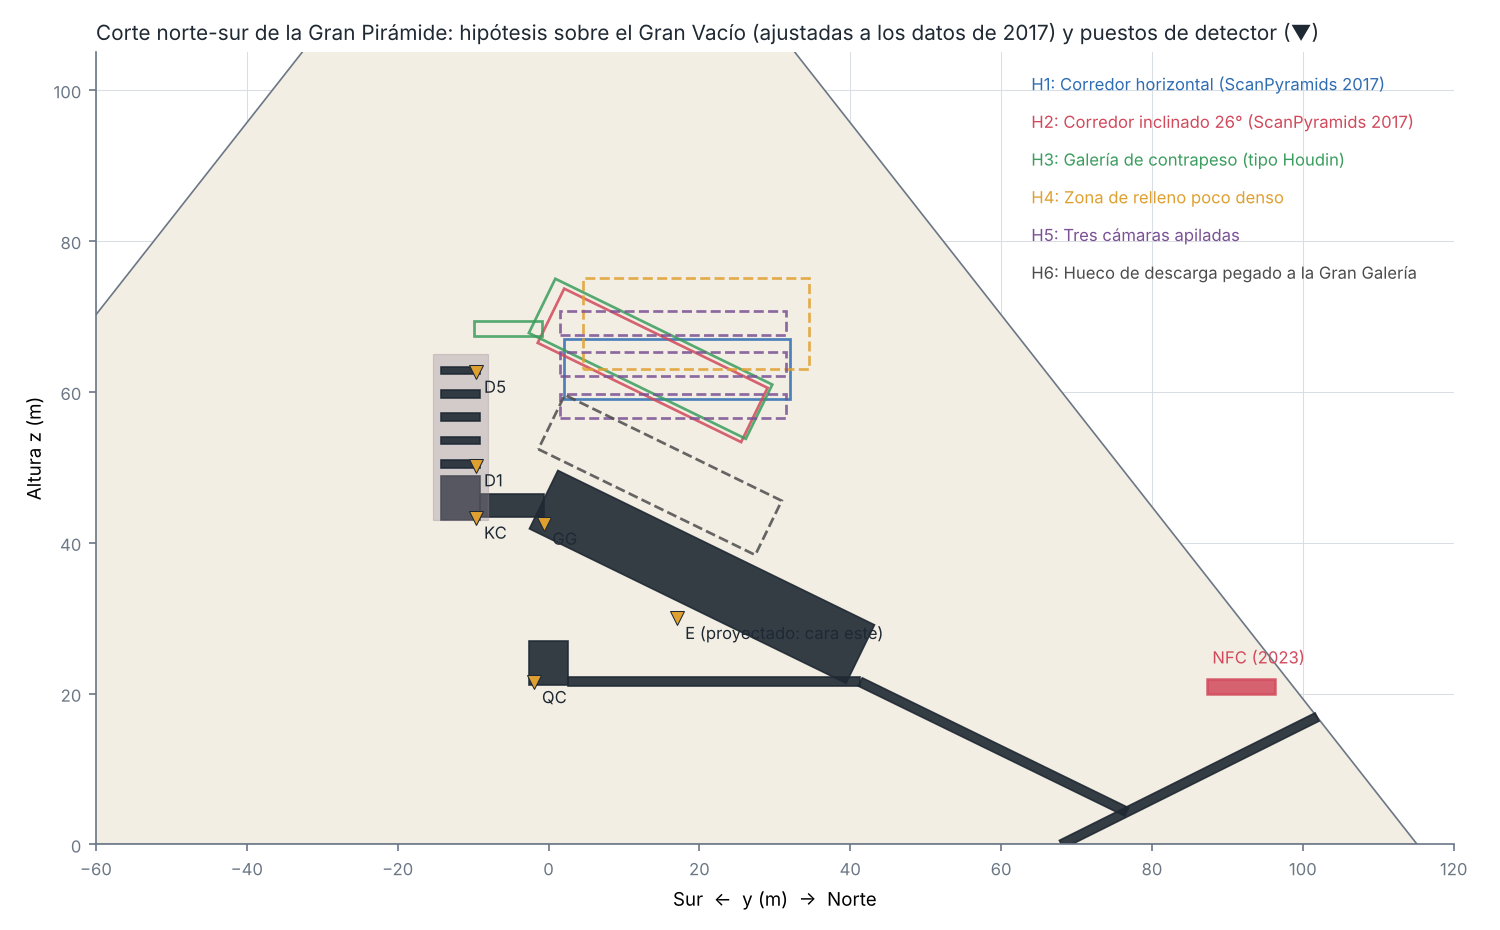
\includegraphics{../figuras/04a_corte_hipotesis.png}
\caption{Hypotheses fitted to the 2017 Queen's Chamber view and
candidate detector positions (▼).}
\end{figure}

We consider five hypotheses:

\begin{itemize}
\tightlist
\item
  H1: a horizontal corridor;
\item
  H2: a corridor inclined at 26°;
\item
  H3: a 26° counterweight gallery joined to the relieving chambers;
\item
  H4: a loose-fill zone;
\item
  H5: stacked low chambers.
\end{itemize}

Each is fitted to mimic the Queen's Chamber view. H1, H2, H3 and H5
remain within 2.3--2.8σ of each other. A relieving void hugging the
Grand Gallery roof is excluded at 29σ, and an open internal spiral ramp
of Houdin's type would have produced a 17--32σ ring that is not seen.

\begin{figure}
\centering
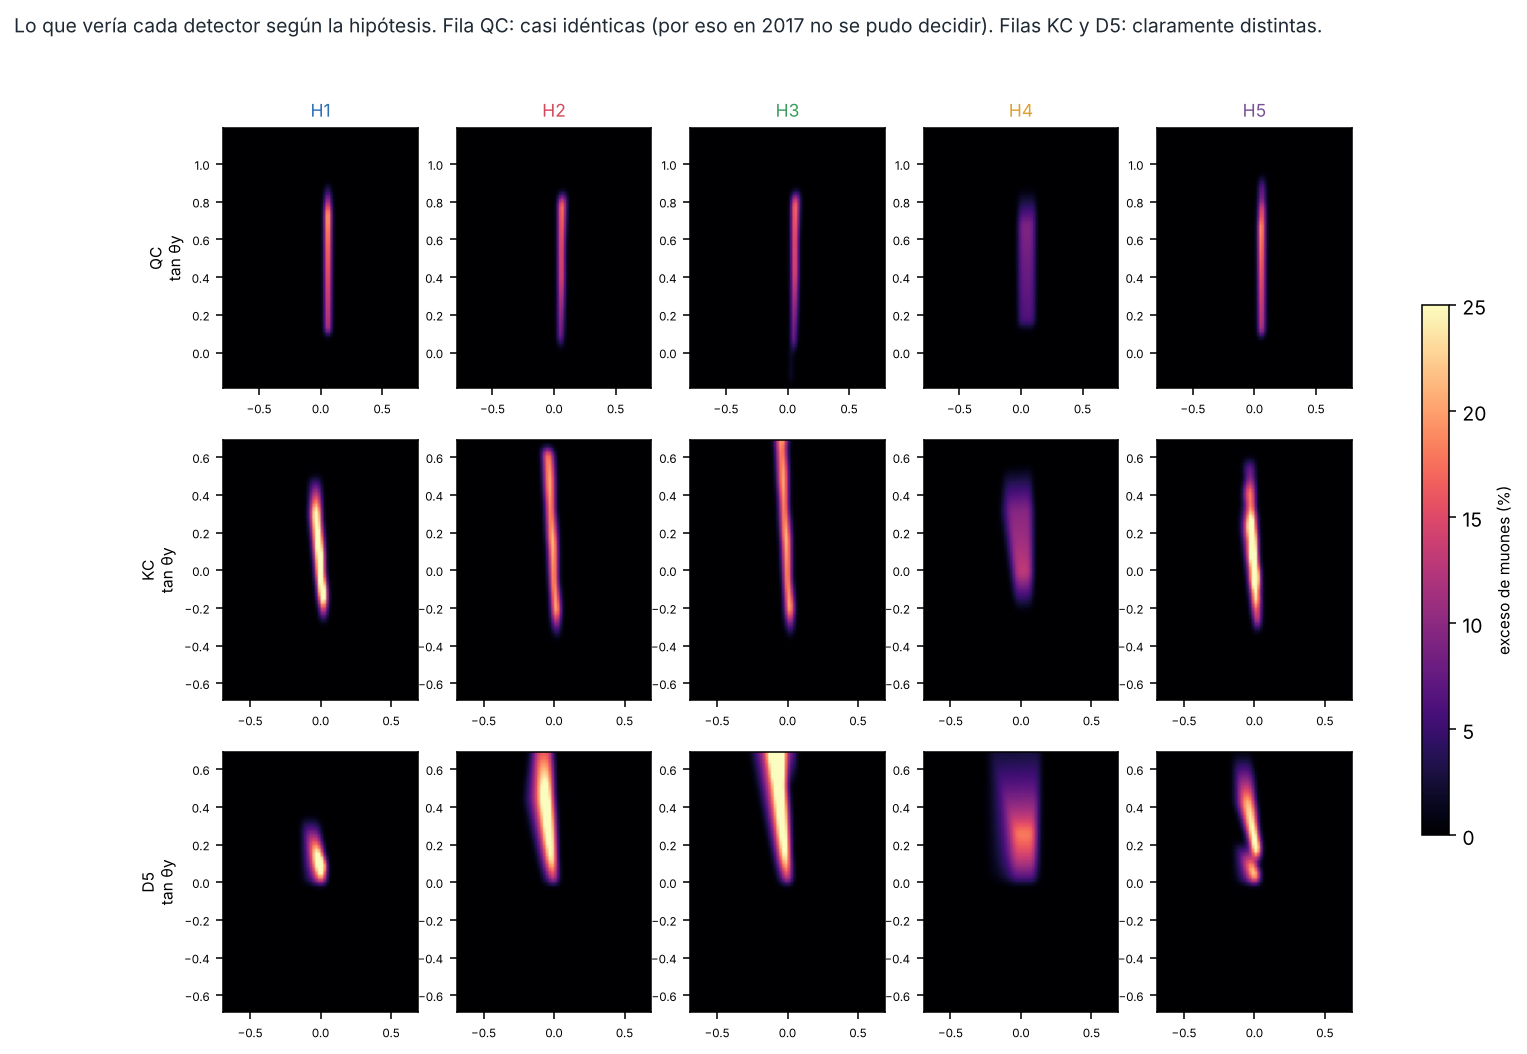
\includegraphics{../figuras/04b_mapas_exceso.png}
\caption{Expected excess maps. Top row: Queen's Chamber (nearly
identical). Middle: King's Chamber. Bottom: Campbell's Chamber.}
\end{figure}

\hypertarget{a-decisive-low-cost-measurement}{%
\section{5. A decisive, low-cost
measurement}\label{a-decisive-low-cost-measurement}}

The test uses a joint fit (Queen's Chamber + new position), with 225
variants per hypothesis (±3 m, cross-section ×0.75--1.25) and profiled
systematics. Blind trials are generated with altered physics --- flux
±10 \% and spectral index ±0.05, limestone 2.35 g/cm³, known chambers
displaced by 1 m. The King's Chamber identifies the true hypothesis in
\textbf{96--98.5 \%} of cases after 60 days (1 m², 25 \% effective
exposure); Campbell's Chamber reaches 97.5 \% in 7 days.

The counterweight interpretation (H3) is the most sensitive to flux
mismodelling: with a grossly wrong spectrum, H2 is misread as H3. We
therefore pre-register four conditions before H3 may be claimed: ≥5σ
against H2, open-sky flux calibration, laser-scan geometry, and a second
position.

\begin{figure}
\centering
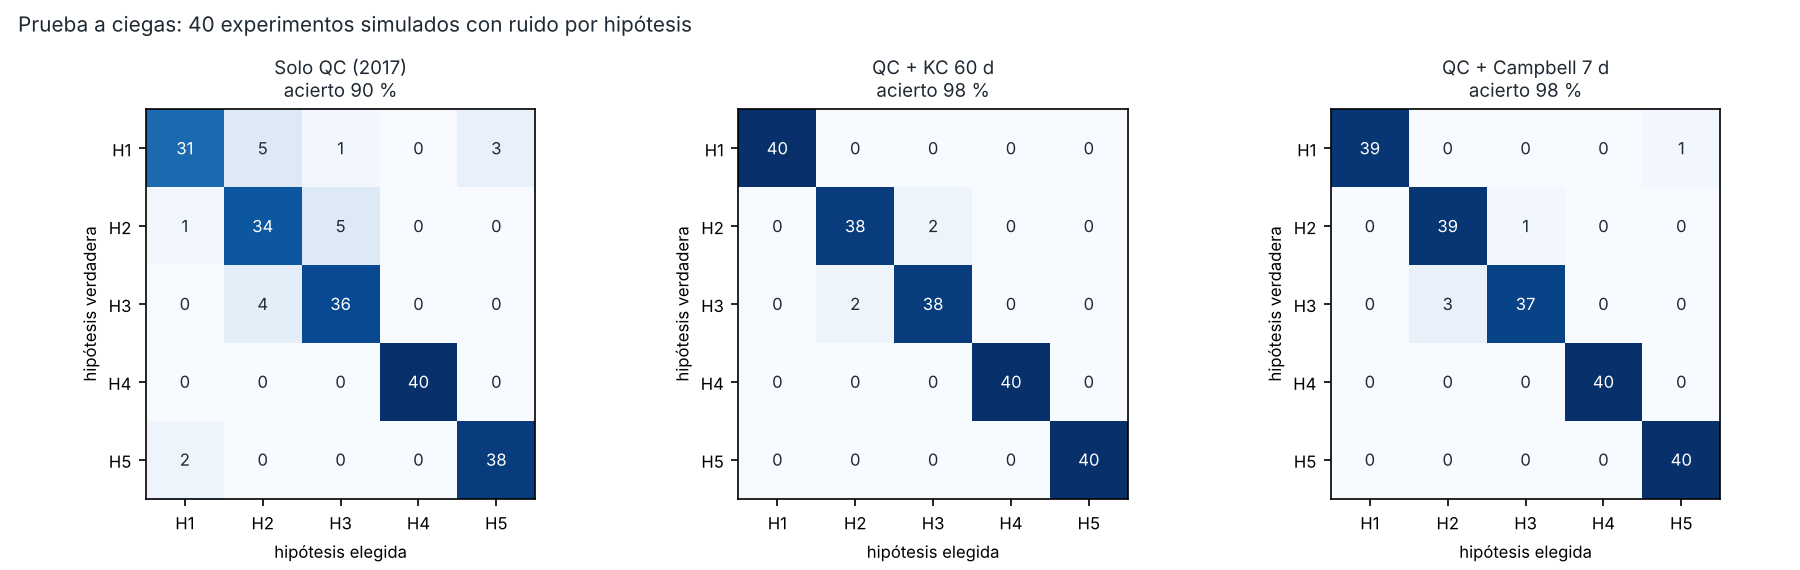
\includegraphics{../figuras/05a_prueba_a_ciegas.png}
\caption{Blind-test confusion matrices.}
\end{figure}

\hypertarget{b.-the-information-limit-cramuxe9rrao}{%
\section{5b. The information limit
(Cramér--Rao)}\label{b.-the-information-limit-cramuxe9rrao}}

For counting data, Var(θ̂) ≥ (F⁻¹)\_jj, where F\_jk = Σ ∂\_jμ\_i ∂\_kμ\_i
/ (μ\_i + f²μ\_i²). Systematics are marginalized.

\begin{longtable}[]{@{}lll@{}}
\toprule\noalign{}
True void & 2017 stereo (NE1 + NE2) & + King's Chamber 60 d \\
\midrule\noalign{}
\endhead
\bottomrule\noalign{}
\endlastfoot
Horizontal & σ(incl.) ≥ 2.5° & ≥ 1.1° \\
Inclined 13° & ≥ 3.3° & ≥ 1.6° \\
Inclined 26° & ≥ 3.0° & ≥ 1.9° \\
\end{longtable}

Blind tests with the stereo configuration give 92 \% accuracy with
\textasciitilde3σ margins (2017 only), and 98.5 \% with 4.3--9σ margins
when 60 days in the King's Chamber are added. Campbell's Chamber sees a
horizontal void almost edge-on; with a 70° zenith cut it adds no
information in that case, so the King's Chamber is the robust choice.

\hypertarget{reanalysis-of-the-published-2017-data}{%
\section{6. Reanalysis of the published 2017
data}\label{reanalysis-of-the-published-2017-data}}

The fits are robust in three respects:

\begin{itemize}
\tightlist
\item
  the void lies on the Grand Gallery axis, x = 7.1--7.5 m vs 7.3 m;
\item
  its centre is at \textasciitilde59--65 m height (emulsions),
  i.e.~38--44 m above the Queen's Chamber;
\item
  its cross-section is \textasciitilde10--13 m².
\end{itemize}

The inclination profile (σ against each angle, errors rescaled by
χ²/ndf):

\begin{longtable}[]{@{}
  >{\raggedright\arraybackslash}p{(\columnwidth - 10\tabcolsep) * \real{0.1667}}
  >{\raggedright\arraybackslash}p{(\columnwidth - 10\tabcolsep) * \real{0.1667}}
  >{\raggedright\arraybackslash}p{(\columnwidth - 10\tabcolsep) * \real{0.1667}}
  >{\raggedright\arraybackslash}p{(\columnwidth - 10\tabcolsep) * \real{0.1667}}
  >{\raggedright\arraybackslash}p{(\columnwidth - 10\tabcolsep) * \real{0.1667}}
  >{\raggedright\arraybackslash}p{(\columnwidth - 10\tabcolsep) * \real{0.1667}}@{}}
\toprule\noalign{}
\begin{minipage}[b]{\linewidth}\raggedright
Data
\end{minipage} & \begin{minipage}[b]{\linewidth}\raggedright
0°
\end{minipage} & \begin{minipage}[b]{\linewidth}\raggedright
10°
\end{minipage} & \begin{minipage}[b]{\linewidth}\raggedright
20°
\end{minipage} & \begin{minipage}[b]{\linewidth}\raggedright
26°
\end{minipage} & \begin{minipage}[b]{\linewidth}\raggedright
35°
\end{minipage} \\
\midrule\noalign{}
\endhead
\bottomrule\noalign{}
\endlastfoot
Emulsions (nominal) & 0.4 & 0.9 & 2.2 & 2.8 & 3.9 \\
Emulsions, without the southern slice & 1.6 & 0.5 & 0.1 & 0.4 & 1.0 \\
KEK alone (detector position free) & 4.3 & 2.5 & 1.0 (18°) & 0.0 &
1.8 \\
\end{longtable}

Under a common geometry the two data sets disagree (Δχ² ≈ 78), and the
disagreement is unchanged for straight, two-segment and two-level
shapes. This indicates a systematic, most plausibly the KEK
normalization to the authors' simulation of known structures or the
hodoscope geometry, which only the original maps can resolve.

\textbf{Our own error.} A first version reported an 18° inclination at
4--6σ, robust to five variations. A leave-one-slice-out test removed it.
We traced it to 26 of 396 bins in which the overlaid fitted curve had
been digitized instead of the data cross.

\hypertarget{the-corner-bottleneck-in-ramp-construction}{%
\section{7. The corner bottleneck in ramp
construction}\label{the-corner-bottleneck-in-ramp-construction}}

\begin{figure}
\centering
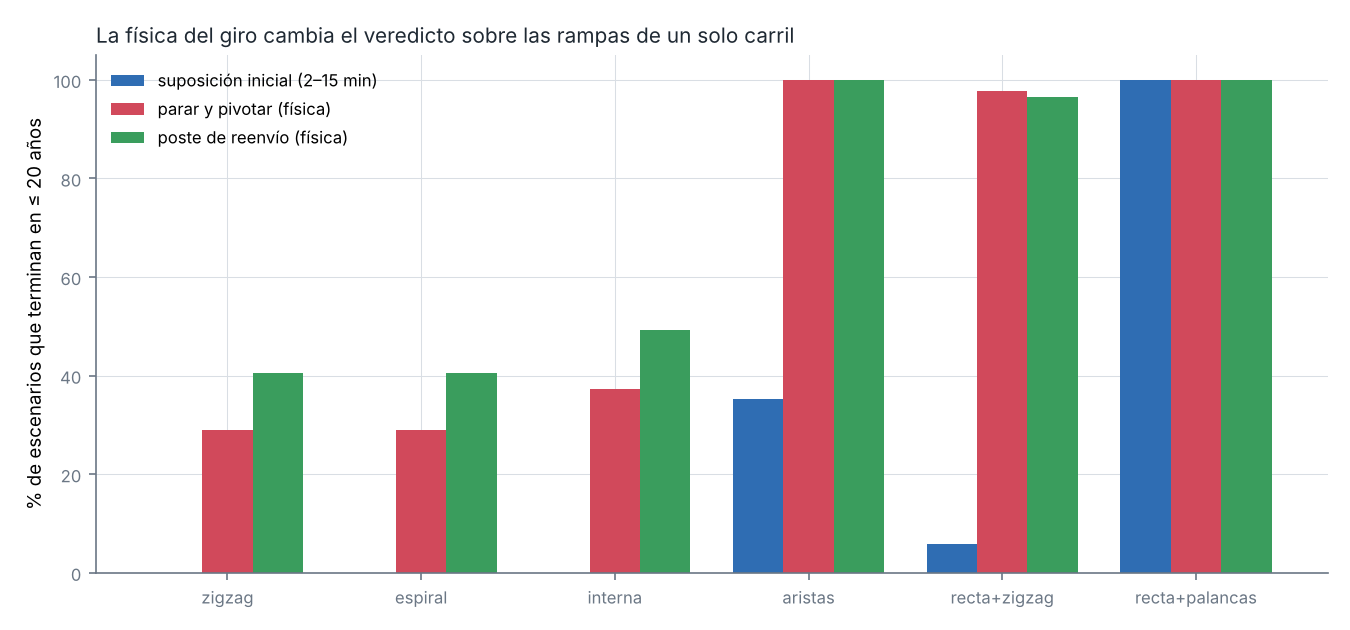
\includegraphics{../figuras/07_giros.png}
\caption{Feasibility (≤20 years) with the initial corner-time assumption
and with physics-derived corner times.}
\end{figure}

Rotating a 2.6 t sledge needs \textasciitilde2.4 kN·m of torque, which
six lever-men supply in seconds. The cost of a corner is the crew's
stop, re-positioning and restart: 0.8--2.8 min in total. A
rope-redirecting post reduces corner occupancy to \textasciitilde0.3
min, at the cost of a capstan factor e\^{}\{μ\_c π/2\} = 1.4--1.9 on
crew size.

\begin{longtable}[]{@{}lll@{}}
\toprule\noalign{}
Model & Median years & Share of scenarios finishing in ≤ 27 years \\
\midrule\noalign{}
\endhead
\bottomrule\noalign{}
\endlastfoot
Single cornered ramp (zigzag, spiral or internal) & 20--23 & 74--85
\% \\
Four edge ramps & --- & 100 \% \\
Straight ramp to 45 m + zigzag & --- & 96--100 \% \\
Straight ramp to 45 m + levers & --- & 96--100 \% \\
\end{longtable}

An earlier version of our model assumed corner times of 2--15 min and
concluded that single ramps were impossible; we withdraw that
conclusion. We propose a 2--3-day experimental-archaeology test with
pre-registered thresholds: stop-and-pivot ≤ 2.1 min per corner, or post
friction μ\_c ≤ 0.4, implies that a single ramp suffices.

\hypertarget{pre-registered-predictions}{%
\section{8. Pre-registered
predictions}\label{pre-registered-predictions}}

The full list is in \texttt{PREDICCIONES.md}, dated in git. The main
ones:

\begin{enumerate}
\def\labelenumi{\arabic{enumi}.}
\tightlist
\item
  From the King's Chamber, the five hypotheses produce distinct
  signatures, separable in ≤ 2 months with 1 m². 1b. A stereo analysis
  of the full 2017 NE1 + NE2 maps prefers the true shape at
  \textasciitilde2--3σ and fixes the void height to ≤ 1 m.
\item
  The void centre lies within ±0.5 m of the Grand Gallery's vertical
  plane, at 56--66 m height, with a cross-section of 10--13 m².
\item
  An open internal spiral ramp does not exist.
\item
  If edge-integrated ramps were used and back-filled with material ≥5 \%
  lighter, an external detector sees helical bands in
  \textasciitilde30--300 days.
\item
  Corner post sockets should exist if the post technique was used.
\end{enumerate}

\hypertarget{limitations}{%
\section{9. Limitations}\label{limitations}}

\begin{itemize}
\tightlist
\item
  No full transport simulation (Geant4); multiple scattering is
  represented by a fitted angular smearing.
\item
  Approximate internal geometry.
\item
  The reanalysis uses digitized figures, not raw data.
\item
  The construction model is a mean-flow model, not an agent-based one.
\end{itemize}

\hypertarget{conclusion}{%
\section{10. Conclusion}\label{conclusion}}

The public data establish where the Big Void is and how large it is, but
not its shape. We identify a cheap, accessible measurement that would
decide among the competing hypotheses, and a simple experiment that
would decide whether a single ramp sufficed. Both are designed so that
their results can prove us wrong.

\hypertarget{references}{%
\section{References}\label{references}}

\begin{itemize}
\tightlist
\item
  Morishima, K. et al.~\emph{Nature} 552, 386--390 (2017).
  arXiv:1711.01576.
\item
  Procureur, S. et al.~\emph{Nat. Commun.} 14, 1144 (2023).
\item
  Reyna, D. hep-ph/0604145 (2006).
\item
  Gaisser, T. K. \emph{Cosmic Rays and Particle Physics} (1990).
\item
  Fall, A. et al.~\emph{Phys. Rev.~Lett.} 112, 175502 (2014).
\item
  Tallet, P. \emph{Les papyrus de la mer Rouge I}, MIFAO 136 (2017).
\item
  Enmarch, R. \& Gourdon, Y. Hatnub ramp (IFAO / University of
  Liverpool, 2018).
\item
  Rosell Roig, V. L. arXiv:2511.06112; \emph{npj Heritage Science}
  (2026).
\item
  Houdin, J.-P. \emph{Khufu: The Secrets Behind the Building of the
  Great Pyramid} (2006).
\item
  Lehner, M. \emph{The Complete Pyramids} (1997).
\item
  Petrie, W. M. F. \emph{The Pyramids and Temples of Gizeh} (1883).
\end{itemize}

\end{document}
